\documentclass[11pt, oneside]{article}   	% use "amsart" instead of "article" for AMSLaTeX format
\usepackage{geometry}                		% See geometry.pdf to learn the layout options. There are lots.
\geometry{letterpaper}                   		% ... or a4paper or a5paper or ... 
%\geometry{landscape}                		% Activate for for rotated page geometry
%\usepackage[parfill]{parskip}    		% Activate to begin paragraphs with an empty line rather than an indent
\usepackage{graphicx}				% Use pdf, png, jpg, or eps� with pdflatex; use eps in DVI mode
								% TeX will automatically convert eps --> pdf in pdflatex		
\usepackage{amssymb}
\usepackage{amsmath}
\usepackage{parskip}


\title{Funky functions}
%\author{The Author}
%\section{}
% \subsection*{R code}
\date{}							% Activate to display a given date or no date

\graphicspath{{/Users/telliott_admin/Dropbox/Tex/png/}}
% \begin{center} 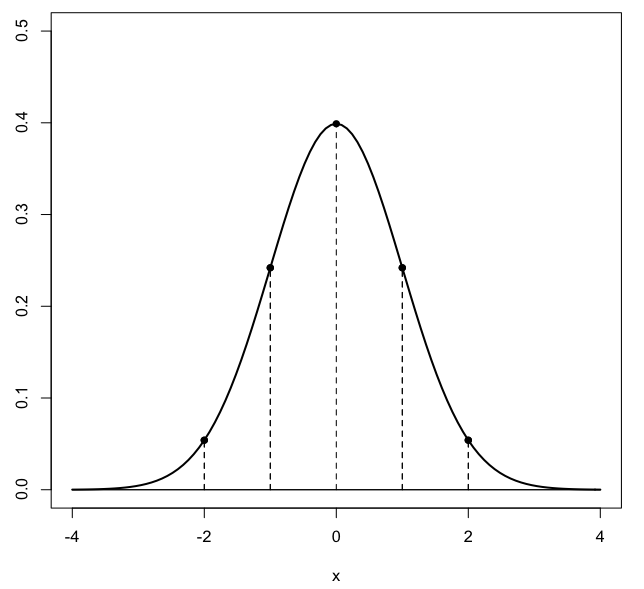
\includegraphics [scale=0.4] {gauss3.png} \end{center}

\begin{document}
\maketitle
\large

A simple approach to calculus is one in which we just try to calculate derivatives and integrals in order to solve problems.  Then, there are more sophisticated approaches in which limits are emphasized, becoming ever more complicated as the discussion becomes more rigorous.  One reason this is needed (at least for mathematicians) is to be able handle functions that are not as well-behaved as $f(x) = x^2$.

Here are some examples:

\[ y = f(x) = \frac{x^2 (x-1)}{x-1} \]
This function acts just like $x^2$ except it has a "hole" in it at $x=1$, where it is undefined.  An exactly equivalent way to write it is

\[
f(x) =
\begin{cases}
x^2 & x \ne 1 \\
\text{undefined} & x = 1
\end{cases}
\]
We say that the limit of $f(x)$ as $x \rightarrow 1$ exists, because the one-sided limits $x \rightarrow 1^+$ and $x \rightarrow 1^-$ both exist \emph{and have the same value}.  It is not necessary for $f(x)$ to be defined at $x=a$ in order for the limit at $f(a)$ to be defined.

Another one is

\[ f(x) = \frac{1}{x^2} \]
This function is not defined at $x=0$

\subsection*{Jumps}

Functions can have jumps.  For example, let $f(x)$ be the greatest integer $\le x$.  So, for example, $f(\pi) = 3$.

\subsection*{One-sided limits not equal}

The function

\[ f(x) = \frac{1}{x} \]
is like $f(x)=1/x$, but it has an additional problem.  As $x$ becomes very close to zero from the right-hand side ($x \rightarrow 0^+$), $f(x)$ becomes infinitely large.  Whereas for $x \rightarrow 0^-$, the function becomes infinitely small.  Since these two one-sided limits are not equal, we say that the limit at $x=0$ does not exist.

\subsection*{Absolute value}

\[ f(x) = | x | \]

\subsection*{Gap}

\[ f(x) = \sqrt{x^2 - 16} \]
This function is simply not defined for $-4 < x < 4$.

\subsection*{Infinite oscillation}

\[ f(x) = \sin \frac{1}{x} \]
The value for $\sin x$ is always $-1 \le \sin x \le 1$, but as $x$ becomes smaller, $1/x$ becomes larger, and since every value of $1/x$ which is an integer multiple of $\pi$ has a sine of $0$ ($\sin n \pi = 0, n = 0, 1, 2 \dots$), the oscillations become faster and faster.

\subsection*{Continuity}

Another important (and subtle) concept is continuity.  Conceptually, a function is continuous over an interval if we can draw the graph of the function \emph{without lifting our pencil from the paper}.











\end{document}  